\documentclass[aspectratio=169,11pt]{beamer}
\usepackage{teaching_slides}
\usepackage{listings}

\lstset{
  language=R,
  basicstyle=\ttfamily\tiny,
  backgroundcolor=\color{gray!5},
  frame=single,
  rulecolor=\color{gray!50},
  keywordstyle=\color{blue!70!black},
  commentstyle=\color{green!40!black},
  stringstyle=\color{orange!90!black},
  columns=flexible,
  keepspaces=true,
  showstringspaces=false,
  breaklines=true
}


\usepackage{inconsolata} % nice monospace font


\title[L11a - Matching]{ Econometrics I}
\subtitle{Lecture 11a: Matching}
\author{Chris Conlon \\NYU Stern}
\date{Fall 2026}

\begin{document}
\frame{\titlepage}

\section{Matching}


\begin{frame}{Recall: Fundamental Problem of Causal Inference}
\begin{columns}[T] % align columns
\begin{column}{.65\textwidth}
Fundamental Problem of Causal Inference
\begin{itemize}
\item We don't observe the \alert{counterfactual} $Y_i(1-D_i)$.
\item For a single individual we either observe $Y_i(1)$ \alert{or} $Y_i(0)$ but never both!
\item Matching says: Find someone with treatment status $1-D_i$ but the same $X_i$ (or \alert{re-weight} your sample)
\begin{itemize}
	\item Assume all selection into treatment is based only on observed $X_i$
	\item Ignore \alert{selection on unobservables}
\end{itemize}
\end{itemize}
\end{column}%
\hfill%
\begin{column}{.33\textwidth}

  \vspace{20pt}
  
  $Y_{i} = D_{i}\cdot Y_{i}(1) + (1-D_{i}) \cdot Y_{i}(0)$\\
  \vspace{20pt}
  \begin{tabular}{ccccc}
    \toprule
    i & $Y_{i}(1)$ &  $Y_{i}(0)$ & $D_{i}$ & $X_{i}$ \\
    \midrule
    1 &     1      &     \alert{?}      &   1   & 3.2 \\
    2 &     0      &     \alert{?}      &   1   & 1.7 \\
    3 &     \alert{?}      &     0      &   0   & 2.5 \\
     & &  $\vdots$ & & \\
    $n$ &     \alert{?}      &     1      &   0   & -1.5 \\    
    \bottomrule
  \end{tabular}
\end{column}%
\end{columns}
\end{frame}

\begin{frame}{Motivating Matching}
Suppose you ran a drug-trial experiment
\begin{itemize}
\item Collected demographic information on each patient (Age, Sex, Education, Income)
\item Flipped a coin to determine treatment status $D_i=1$ if \textit{Heads}, $D_i=0$ if \textit{Tails}. 
\item First course of action: Construct a \alert{covariate balance table}.
\item If your control group is 70\% male and your treatment group is 70\% female, should you compare differences in means?
\begin{itemize}
	\item Probably we wanted to compare treated males to control males, and treated females to control females.
	\item Otherwise, are we learning about the difference between sexes, or the effect of treatment?
\end{itemize}
\end{itemize}
\end{frame}


\begin{frame}{Balance Table: Examples (see \texttt{cobalt} Package)}
\begin{columns}
\begin{column}{0.5\textwidth}
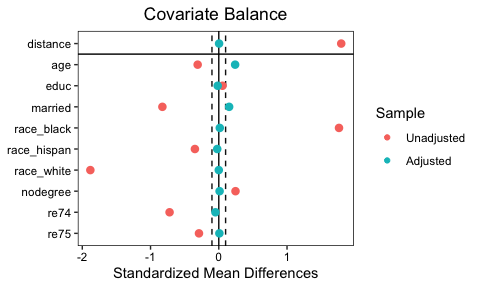
\includegraphics[width=\textwidth]{resources/balance_plot.png}
\end{column}
\begin{column}{0.5\textwidth}
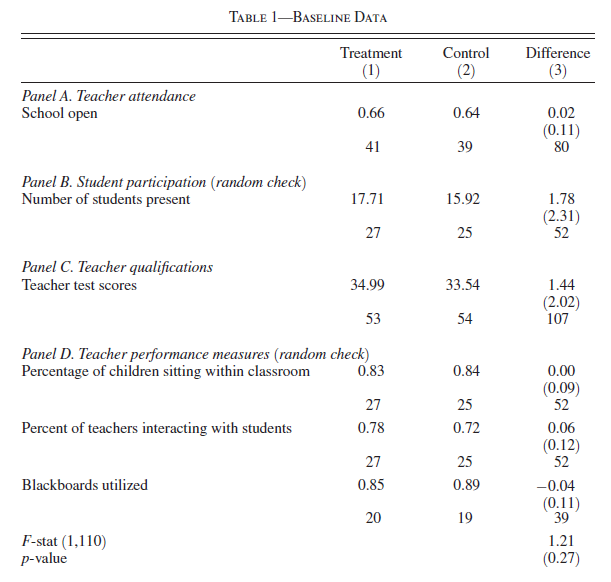
\includegraphics[width=\textwidth]{resources/duflo-balance-table.png}
\end{column}
\end{columns}
\end{frame}


\begin{frame}{Checking Balance: Standardized Differences}
For each covariate $k$, compare the treated and control means in units of its standard deviation:
\begin{align*}
d_k=\frac{\bar x_{k,1}-\bar x_{k,0}}{\sqrt{\left(s^2_{k,1}+s^2_{k,0}\right)/2}}
\end{align*}
\begin{itemize}
\item \alert{Not a $t$-test.} A $t$-statistic grows with $\sqrt{n}$: trivial imbalance is ``significant'' in a big sample,
and matching or trimming can raise $p$-values just by dropping observations.
\item Rules of thumb: $|d_k| < 0.1$ is well balanced (Austin 2009); Imbens and Rubin (2015) worry above $0.25$.
Also check variance ratios $s^2_{k,1}/s^2_{k,0}$: outside $[0.5, 2]$ is a warning.
\item Report $d_k$ before and after matching or weighting, for every covariate (and key squares and interactions).
The left panel on the previous slide is exactly this: \texttt{cobalt::love.plot()}.
\item Balance on observables is necessary, not sufficient: it says nothing about unobservables.
\end{itemize}
\end{frame}


\begin{frame}
\frametitle{Matching}
\begin{itemize}
\item Formally the key assumption is the \alert{Conditional Independence Assumption (CIA)}
\begin{eqnarray*}
\{Y_i(1),Y_i(0)\}  \perp D_i | X_i
\end{eqnarray*}
\item Once we know $X_i$ allocation to treatment $D_i$ is as if it is random.
\item The only difference between treatment and control is composition $f(X_i | D_i)$ of the sample.
\begin{itemize}
\item Re-weight so distribution of $X_i$ is the same for both groups $ X_i | D_i \sim X_i$ then we assume all other differences are irrelevant and can just compare means.
\item Unobservables that affect outcomes are \alert{unrelated to treatment} conditional on $X_i$.
\end{itemize}
\end{itemize}
\end{frame}

\begin{frame}{Simple Matching in Practice}
For each observation $i$ in the \alert{treated group}, find $\mathcal{C}_i$ the set of observations in the \alert{control group} with the same $X_i$:
\begin{align*}
ATT = \frac{1}{N_T} \sum_{i=1}^{N_T}\left(Y_i(1)-\frac{1}{|\mathcal{C}_i|} \sum_{j \in \mathcal{C}_i} Y_j(0)\right)
\end{align*}
Some issues:
\begin{itemize}
	\item For each observation $|\mathcal{C}_i|$ may be a different size (including zero!). This can make the variance a bit unpredictable.	
	\item Finding \alert{exact matches} gets harder as $\dim(X_i)$ grows.
\end{itemize}
\end{frame}



\begin{frame}
\frametitle{Why would this work?}
\small
Let  $F^{1}(x)$ be the distribution of characteristics in the treatment group, we can define the ATT as 
\begin{align*}
&\mathbb{E}[Y(1) - Y(0) \mid D =1] =\mathbb{E}_{F^1(x)} \left[\mathbb{E}(Y(1) -Y(0) \mid D=1,X) \right]  \text{ L.I.E. }\\
=&\mathbb{E}_{F^1(x)} [\mathbb{E}(\alert{Y(1)} \mid D=1,X)] -  \mathbb{E}_{F^1(x)} [\mathbb{E}(\alert{Y(0)} \mid D=1,X)] \text{ linearity } 
\end{align*}
The first part we observe directly:
\begin{align*}
&=\mathbb{E}_{F^1(x)} [\mathbb{E}(Y(1) \mid D=1,X)] 
\end{align*}
But the counterfactual mean is not observed!
\begin{align*}
&=\mathbb{E}_{F^1(x)} [\mathbb{E}(Y(0) \mid D=1,X)] 
\end{align*}
But conditional independence does this for us:
\begin{align*}
 \mathbb{E}_{F^1(x)} [\mathbb{E}(Y(0) \mid \alert{D=1},X)]  =  \mathbb{E}_{F^1(x)} [\mathbb{E}(Y(0) \mid \alert{D=0},X)] 
\end{align*}
(For the ATT we only need $Y(0) \perp D \mid X$ and $P(X)<1$.)
\end{frame}



\begin{frame}
\frametitle{Aside: Matching and OLS}
\begin{itemize}
\item Think about
\begin{eqnarray*}
Y_i  = \alpha + \beta D_i + u_i
\end{eqnarray*}
\item Assume that $\E(u_i \mid D_i,X_i) = \E(u_i \mid X_i) = \gamma_0 + \gamma X_i$ (conditional mean independence with a linear control function)
\item Then we can get $\beta$ consistently (but not other variables) by running the following:
\begin{eqnarray*}
Y_i = \alpha + \beta D_i + \gamma X_i + v_i
\end{eqnarray*}
\item Again we are in the homogeneous treatment world
\end{itemize}
\end{frame}



\begin{frame}
\frametitle{Higher Dimensions}
So matching works in dimension 1. But what if $\dim(X) > 1$?
\begin{itemize}
\item True high-dimensional matching may be infeasible: there may be no controls with the same $X_i$, so we cannot build weights $w(x)$ with $f(x \mid D=1) = w(x)\, f(x \mid D=0)$ from the sample.
\item One solution is the nearest-neighbor approach in Abadie and Imbens (2006) (later on).
%\item This is still cursed in that our nearest neighbors get further away as the dimension grows.
\item Suppose instead we had a \alert{sufficient statistic}
\end{itemize}
\end{frame}


\begin{frame}{Propensity Score}
\begin{itemize}
\item Rosenbaum and Rubin (1983) propose the \alert{propensity score} as a sufficient statistic
\begin{align*}
\Pr(D_i  = 1 \mid X_i) \equiv P(X_i)
\end{align*}
\item Idea: avoid high-dimensional problems by matching on $P(X_i)$.
\item They prove that the propensity score and any function of $X$, $b(X)$ which is finer serves as a \alert{balancing score}.
\item Finer implies that:
\begin{align*}
b(X^1) = b(X^2) &\implies P(X^1) = P(X^2)\\
P(X^1) = P(X^2) & \nRightarrow  b(X^1) = b(X^2)
\end{align*}
\end{itemize}
\end{frame}


\begin{frame}
\frametitle{Propensity Score}
\begin{itemize}
\item Main Result: If treatment assignment is strongly ignorable conditional on $X$ (CIA) then it is strongly ignorable $Y(1),Y(0) \perp D \mid b(X)$ given any balancing score $b(X)$ including the propensity score:
\begin{align*}
\Pr(D=1 \mid Y(1), Y(0),P(X))&= \E[\Pr(D=1\mid Y(1),Y(0),X) \mid Y(1),Y(0),P(X)] \\
&= \E[P(X) \mid Y(1),Y(0),P(X) ] = P(X) \qquad \text{(CIA in the second step)}
\end{align*}
\item Also we require that $0 < P(X) < 1$ at each $X$ which is known as the \alert{support condition}.
\item The theorem implies that given $P(X)$ we have as if random assignment.
\end{itemize}
\end{frame}


\begin{frame}
\frametitle{Propensity Score}
Just like in the matching case the problem arises because we do not observe the counterfactual mean:
\begin{align*}
 \E_{F^1(x)} [\E(Y(0) \mid D=1,X)] 
\end{align*}
With conditional independence and the propensity score:
\begin{align*}
 \E_{F^1(x)} [\E(Y(0) \mid D=1,X)]  &=  \E_{F^1(x)} [\E(Y(0) \mid D=0,X)] \\
 &=  \E_{F^1(x)} [\E(Y(0) \mid D=0, \alert{P(X)})] 
\end{align*}
\end{frame}

\begin{frame}
\frametitle{Propensity Score}
\begin{itemize}
\item Instead of matching on high dimensional $X$ we can now match on a one-dimensional propensity score.
\item Thus the propensity score provides \alert{dimension reduction}
\item We still have to estimate the propensity score which is a high dimensional problem!
\begin{itemize}
\item An easy way would be to use $\pi(x)=P(x)$ from logit or probit.
\item To be fancy, include polynomial interactions in $X_i$.
\end{itemize}
\item People often match on \alert{caliper} of propensity score $d_{ij} = \lvert\pi(x_i) - \pi(x_j)\rvert$ where $d_{ij} < c$
\begin{itemize}
\item Compare to other $x_j$ with similar $\pi(x_i)=0.34$ and $\pi(x_j)=0.32$.
\end{itemize}

\end{itemize}
\end{frame}





\begin{frame}{Kernel Matching}
How do we implement?
\begin{itemize}
\item Kernels are an obvious choice
\begin{align*}
\widehat{ATT} = \frac{1}{N_1} \sum_{i: D_i=1} \left[Y_i - \frac{\sum_{j: D_j=0} Y_j \cdot \mathcal{K}\left(\frac{P(X_i) - P(X_j)}{h} \right) }{\sum_{s: D_s=0}  \mathcal{K}\left(\frac{P(X_i) - P(X_s)}{h} \right)}   \right]
\end{align*}
 where $N_1$ is the sample size of the treatment group \\
 and $\mathcal{K}(u)$ is a valid Kernel weight with bandwidth $h$ (people tend to use Gaussian Kernels here)
\item As your propensity score gets further away from observation $i$ you get less weight
\item As $h \rightarrow 0$  (or $\sigma_h$) the window gets smaller and we use fewer neighbors.
\end{itemize}
\end{frame}


\begin{frame}
\frametitle{Related: Inverse Probability Weighting}
\begin{itemize}
\item Calculate a smoothed estimate of the treatment probability $\pi(x) = \Pr(D_i =1 \mid x)$. (Logit or Probit)
\begin{align*}
ATE = \frac{1}{n}\sum_{t \in \text{Treatment}} \frac{y_t}{\pi(x_t)} - \frac{1}{n} \sum_{s \in \text{Control}} \frac{y_s}{1-\pi(x_s)}
\end{align*}
\item How to get $\pi(x)$? Run a logit or probit.
\item Normalize the weights within each arm (H\'ajek):
\begin{align*}
\widehat{ATE}=\frac{\sum_i D_iY_i/\pi(x_i)}{\sum_i D_i/\pi(x_i)}-\frac{\sum_i (1-D_i)Y_i/(1-\pi(x_i))}{\sum_i (1-D_i)/(1-\pi(x_i))}
\end{align*}
\item Helps with very large weights; also consider trimming to $0.1\le\pi(x)\le0.9$ (Crump et al.\ 2009).
\end{itemize}
\end{frame}


\begin{frame}{Doubly Robust: Augmented IPW (AIPW)}
\small
Combine an outcome model $\widehat\mu_d(x)=\widehat{\E}[Y\mid D=d,X=x]$ with the propensity score:
\begin{align*}
\widehat{ATE}_{AIPW}=\frac{1}{n}\sum_{i=1}^n\left[\widehat\mu_1(X_i)-\widehat\mu_0(X_i)
+\frac{D_i\left(Y_i-\widehat\mu_1(X_i)\right)}{\widehat\pi(X_i)}
-\frac{(1-D_i)\left(Y_i-\widehat\mu_0(X_i)\right)}{1-\widehat\pi(X_i)}\right]
\end{align*}
\begin{itemize}
\item A regression estimate plus an IPW correction built from its residuals.
\item \alert{Doubly robust}: consistent if \emph{either} $\widehat\pi$ \emph{or} $\widehat\mu_d$ is correctly specified. If $\widehat\mu_d$ is
right, the correction has mean zero; if $\widehat\pi$ is right, the correction removes $\widehat\mu_d$'s bias.
\item With both right, it attains the semiparametric efficiency bound (Robins, Rotnitzky and Zhao 1994; Hahn 1998).
\item Still needs CIA and overlap: it does not fix unobserved confounding, and small $\widehat\pi$ still means big weights.
\item The building block of double/debiased ML (Chernozhukov et al.\ 2018): flexible $\pi$, $\mu_d$ with cross-fitting. In R: \texttt{grf::average\_treatment\_effect()}, \texttt{DoubleML}.
\end{itemize}
\end{frame}


\begin{frame}
\frametitle{IPW vs Propensity Score: What's the Difference?}
\begin{columns}
\begin{column}{.5\textwidth}
Propensity Scores
\begin{itemize}
	\item Find individual with similar $p(X)$
	\item Excludes unmatched participants
	\item Creates a balanced \alert{sub-sample}
	\item Can be sensitive to the choice of matching algorithm
	\item With enough data can compute $\E[Y_i(1)-Y_i(0) \mid P(X_i)]$
\end{itemize}
\end{column}
\begin{column}{.5\textwidth}
Inverse Probability Weights
\begin{itemize}
	\item Reweights the entire sample
	\item Keeps all participants
	\item Creates a pseudo-population
	\item Can be sensitive to extreme weights
	\item We only compute ATE or ATT
\end{itemize}
\end{column}
\end{columns}
\end{frame}





\begin{frame}{Other approaches in high dimensions}
\begin{itemize}
\item Given two vectors $\mathbf{x}$ and $\mathbf{y}$, how to choose $d(\mathbf{x},\mathbf{y})$ the \alert{distance} function?
\item Papers mostly use \alert{Mahalanobis distance}: $d(\mathbf{x},\mathbf{y}) = (\mathbf{x}-\mathbf{y}) \Sigma^{-1} (\mathbf{x}-\mathbf{y})'$.
\begin{itemize}
\item Quadratic distance with inverse covariance matrix as ``weights''.
\item Reduces to Euclidean distance when $\Sigma=I$ (standardized Euclidean for diagonal $\Sigma$).
\end{itemize}
\item Older papers use \alert{caliper matching} anything within $\norm{\mathbf{x_s} -\mathbf{x_t}}<b$ is a match
\begin{itemize}
\item Number of matches varies from observation to observation.
\item Variance can be unpredictable: some $(\mathbf{y_i},\mathbf{x_i})$ have many matches, others have none
\item Some obs may have nothing within $\norm{\mathbf{x_s} -\mathbf{x_t}}<b$? Drop these?
\item Probably avoid this unless you have a good reason...
\end{itemize}
\item Let's explore \alert{k Nearest Neighbor Matching} (kNN)
\end{itemize}
\end{frame}



\begin{frame}{Nonparametric $k$-NN Matching: Abadie and Imbens (2006)}
For each observation $i$, we observe $Y_i(D_i)$; compute a \alert{counterfactual} $\hat{Y}_i(1-D_i)$:
\begin{align*}
\begin{array}{l}
\widehat{Y}_{i}(0)=\left\{\begin{array}{cl}
Y_{i} & \text { if } D_{i}=0 \\
\frac{1}{\# \mathcal{J}_{M}(i)} \sum_{l \in \mathcal{J}_{M}(i)} Y_{l} & \text { if } D_{i}=1
\end{array}\right. \\
\widehat{Y}_{i}(1)=\left\{\begin{array}{cc}
\frac{1}{\# \mathcal{J}_{M}(i)} \sum_{l \in \mathcal{J}_{M}(i)} Y_{l} & \text { if } D_{i}=0 \\
Y_{i} & \text { if } D_{i}=1
\end{array}\right.
\end{array}
\end{align*}
\begin{itemize}
\item $\# \mathcal{J}_{M}(i)$ is the number of matches for $i$ of opposite treatment assignment $D_l =1-D_i$.
\item $d_M(i)$ is the distance to the $M$-th closest unit with $D_l=1-D_i$; $\mathcal{J}_{M}(i)=\{l: D_l=1-D_i,\ \norm{X_l-X_i}\le d_M(i)\}$.
\item If there are ties $\# \mathcal{J}_{M}(i) > M$.
\item This is just $k$-NN matching.
\end{itemize}
\end{frame}



\begin{frame}{Nonparametric $k$-NN Matching: Abadie and Imbens (2006)}
Each observation $i$ gets a weight based on how often it is used as a match for other observations $l$:
\begin{align*}
K_{M}(i)=\sum_{l=1}^{N} 1\left\{i \in \mathcal{J}_{M}(l)\right\} \frac{1}{\# \mathcal{J}_{M}(l)}
\end{align*}
 Observations used in lots of matches get more weight. $\sum_{i=1}^N K_{M}(i) = N$.\\
 
This is just a weighted average of $Y_i$ values (aka a \alert{kernel}!):
\begin{align*}
ATE_M=\frac{1}{N} \sum_{i=1}^{N}\left[ \widehat{Y}_{i}(1)-\widehat{Y}_{i}(0)\right]=\frac{1}{N} \sum_{i=1}^{N} \underbrace{\left(2 D_{i}-1\right)\left[1+K_{M}(i)\right]}_{w_{i,M}} Y_{i}
\end{align*}
\end{frame}


\begin{frame}{Nonparametric $k$-NN Matching: Alternatives}
Different weighting schemes give different parameters:
\begin{align*}
ATE_M&=\frac{1}{N} \sum_{i=1}^{N} \left(2 D_{i}-1\right)\left[1+K_{M}(i)\right] \cdot Y_{i} \\
ATT_M&=\frac{1}{N_1}\sum_{i=1}^{N} \left[D_{i}-(1-D_i) \cdot K_{M}(i)\right] \cdot  Y_{i}\\
ATUT_M&=\frac{1}{N_0}\sum_{i=1}^{N} \left[D_{i}\cdot K_{M}(i) -(1-D_i) \right] \cdot Y_{i}
\end{align*}
\end{frame}



\begin{frame}{Nonparametric $k$-NN Matching: Bias Correction (Abadie and Imbens 2011)}
We can use weighted least squares to adjust the predictions $\hat{Y}_i(D_i)$:
\begin{align*}
\left(\widehat{\beta}_{t, 0}, \widehat{\beta}_{t, 1}\right)=\operatorname{argmin}_{\left\{\beta_{t, 0}, \beta_{t, 1}\right\}} \sum_{i: D_{i}=t} K_{M}(i)\left(Y_{i}-\beta_{t, 0}-\beta_{t, 1}^{\prime} X_{i}\right)^{2}
\end{align*}
Where $\widehat{\mu}_t(x)=\widehat{\beta}_{t,0}+\widehat{\beta}_{t,1}'x$ are the fitted regression functions for treatment ($t=1$) and control ($t=0$).
\begin{align*}
\tilde{Y}_{i}(0)=\left\{\begin{array}{cc}
Y_{i} & \text { if } D_{i}=0 \\
\frac{1}{\# \mathcal{J}_{M}(i)} \sum_{l \in \mathcal{J}_{M}(i)}\left\{Y_{l}+\widehat{\mu}_{0}\left(X_{i}\right)-\widehat{\mu}_{0}\left(X_{l}\right)\right\} & \text { if } D_{i}=1
\end{array}\right. \\
\tilde{Y}_{i}(1)=\left\{\begin{array}{cc}
\frac{1}{\# \mathcal{J}_{M}(i)} \sum_{l \in \mathcal{J}_{M}(i)}\left\{Y_{l}+\widehat{\mu}_{1}\left(X_{i}\right)-\widehat{\mu}_{1}\left(X_{l}\right)\right\} & \text { if } D_{i}=0 \\
Y_{i} & \text { if } D_{i}=1
\end{array}\right.
\end{align*}
So that the ATE is given by: $ATE_M=\frac{1}{N} \sum_{i=1}^{N}\left\{\tilde{Y}_{i}(1)-\tilde{Y}_{i}(0)\right\}$
\end{frame}







\begin{frame}{Implementation}
\begin{itemize}
\item Base case is easy enough to do on your own using a canned $k$-NN package.
\item Even regression/bias adjustment is pretty easy
\item Computing ATE, ATT, ATUT is relatively straightforward on the matched sample
\item \texttt{MatchIt} in \texttt{R} (Ho, Imai, King and Stuart) or \texttt{nnmatch} in Stata (Abadie et al.)
\item Documentation here is pretty good: \url{https://scholar.harvard.edu/files/imbens/files/sjpdf-1.html_.pdf}.
\end{itemize}
\end{frame}



% \begin{frame}
% \frametitle{Kernel Matching}
% \begin{itemize}
% \item The usual caveats apply: $h$ determines the \alert{bias-variance} tradeoff
% \item Choice of Kernel effects finite-sample properties
% \item Here the \alert{common support} is important. We can only learn about cases where $P(X) \neq 1$ and $P(X) \neq 0$. If you always get treated (or not-treated) we cannot learn from this observation.
% \item We also have to be careful in choosing $X$ so as not to violate CIA (too many $X$'s , too few $X$'s) $\rightarrow$ have to think carefully!
% \item If you use propensity scores you will need a slide convincing us you have thought about why CIA holds for you!
% \end{itemize}
% \end{frame}



% \begin{frame}
% \frametitle{Gotcha!}
% \small
% Under CIA we know
% \begin{eqnarray*}
% G(Y(1),Y(0) | X, T) = G(Y(1),Y(0) | X)
% \end{eqnarray*}
% Suppose we add in $Z$, then we require that:
% \begin{eqnarray*}
% G(Y(1),Y(0) | X, Z, T) = G(Y(1),Y(0) | X, Z)
% \end{eqnarray*}
% \begin{eqnarray*}
% G(Y(1),Y(0) | X, T) = \int G(Y(1),Y(0) | X, Z, T) dF(Z | X,T) \\
% = G(Y(1),Y(0) | X)
% \end{eqnarray*}
% where the last part follows by CIA.
% \begin{itemize}
% \item Thus each element can depend on $T$ conditional on $Z,X$ but the average may not.
% \item Mindless applications of matching can give you biased results!
% \end{itemize}
% \end{frame}





\section{Case Study}

\begin{frame}
\frametitle{A Matching Example}
Here is an example where I found that matching was helpful in my own work with Julie Mortimer:
\begin{itemize}
\item We ran a randomized experiment where we removed Snickers bars from around 60 vending machines in office buildings in downtown Chicago.
\item We have a few possible control groups:
\begin{enumerate}
\item Same vending machine in other weeks (captures heterogeneous tastes in the cross section)
\item Other vending machines in the same week (might capture aggregate shocks, ad campaigns, etc.)
\end{enumerate}
\item We went with \#1 as \#2 was not particularly helpful.
\end{itemize}
\end{frame}

\begin{frame}
\frametitle{A Matching Example}
Major problem was that there was a ton of heterogeneity in the overall level of (potential) weekly sales which we call $M_t$.
\begin{itemize}
\item Main source of heterogeneity is how many people are in the office that week, or how late they work.
\item Based on total sales our average over treatment weeks was in the 74th percentile of all weeks.
\item This was after removing a product, so we know sales should have gone down!
\item How do we fix this without running the experiment for an entire year?
\item Can't use shares instead of quantities. Why?
\end{itemize}
\end{frame}

\begin{frame}{Sales over Time}
\begin{center}
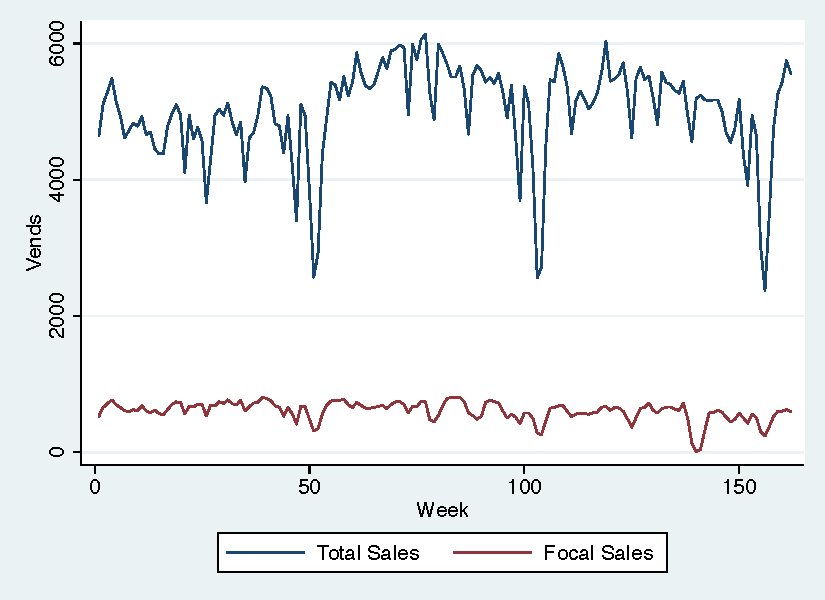
\includegraphics[width=4in]{./resources/figure1.pdf}
\end{center}
\end{frame}

\begin{frame}
\frametitle{A Matching Example}
Ideally we could just observe $M_t$ directly and use that as our matching variable $X$
\begin{itemize}
\item We didn't observe it directly and tried a few different measures:
\begin{itemize}
\item Sales at the soda machine next to the snack machine
\item Sales of salty snacks at the same machine (not substitutes for candy bars).
\item We used k-NN with $k=4$ to select control weeks -- notice we re-weight so that overall sales are approximately the same (minus the removed product).
\end{itemize}
\item We also tried a more structured approach:
\begin{itemize}
\item Define control weeks as valid IFF
\item Treatment-week total sales are weakly lower than the control week's total
\item but no lower than the control week's total minus its Snickers sales.
\end{itemize}
\end{itemize}
\end{frame}


\begin{frame}
\begin{table}
\begin{center}
\tiny
\label{tab:nonparam}
\begin{tabular}{|l|rrrcrrcr|}
\hline
 & Control  & Control & Treatment& \hspace{-0.3in}& Treatment & Mean & \hspace{-0.3in} & \\
Product & Mean &  \%ile & Mean& \hspace{-0.3in} & \%ile &  Difference & \hspace{-0.3in}& \% $\Delta$\\
\hline \hline
\multicolumn{9}{|l|}{\emph{Vends}} \\ \hline
Peanut M\&Ms&359.9&73.6&478.3&\hspace{-0.3in}*&99.4&118.4& \hspace{-0.3in}*&32.9\\
Twix Caramel&187.6&55.3&297.1&\hspace{-0.3in}*&100.0&109.5& \hspace{-0.3in}*&58.4\\
Assorted Chocolate&334.8&66.7&398.0&\hspace{-0.3in}*&95.0&63.2& \hspace{-0.3in}*&18.9\\
Assorted Energy&571.9&63.5&616.2& \hspace{-0.3in}&76.7&44.3 & \hspace{-0.3in} &7.8\\
Zoo Animal Cracker&209.1&78.6&243.7&\hspace{-0.3in}*&98.1&34.6& \hspace{-0.3in}*&16.5\\
Salted Peanuts&187.9&70.4&216.3&\hspace{-0.3in}*&93.7&28.4 & \hspace{-0.3in} &15.1\\
Choc Chip Famous Amos&171.6&71.7&193.1&\hspace{-0.3in}*&95.0&21.5& \hspace{-0.3in}*&12.5\\
Ruger Vanilla Wafer&107.3&59.7&127.9& \hspace{-0.3in}&78.6&20.6& \hspace{-0.3in}*&19.1\\
Assorted Candy&215.8&43.4&229.6& \hspace{-0.3in}&60.4&13.7& \hspace{-0.3in}&6.4\\
Assorted Potato Chips&279.6&64.2&292.4&\hspace{-0.3in}*&66.7&12.8& \hspace{-0.3in}&4.6\\
Assorted Pretzels&548.3&87.4&557.7&\hspace{-0.3in}*&88.7&9.4& \hspace{-0.3in}&1.7\\
Raisinets&133.3&66.0&139.4& \hspace{-0.3in}&74.2&6.1& \hspace{-0.3in}&4.6\\
Cheetos&262.2&60.1&260.5& \hspace{-0.3in}&58.2&-1.8& \hspace{-0.3in}&-0.7\\
Grandmas Choc Chip&77.9&51.3&72.5& \hspace{-0.3in}&37.8&-5.4& \hspace{-0.3in}&-7.0\\
Doritos&215.4&54.1&203.1& \hspace{-0.3in}&39.6&-12.3& \hspace{-0.3in}*&-5.7\\
Assorted Cookie&180.3&61.0&162.4& \hspace{-0.3in}&48.4&-17.9& \hspace{-0.3in}&-10.0\\
Skittles&100.1&62.9&75.1&\hspace{-0.3in}*&30.2&-25.1& \hspace{-0.3in}*&-25.0\\
Assorted Salty Snack&1382.8&56.0&1276.2&\hspace{-0.3in}*&23.3&-106.7& \hspace{-0.3in}*&-7.7\\
Snickers&323.4&50.3&2.0&\hspace{-0.3in}*&1.3&-321.4& \hspace{-0.3in}*&-99.4\\ \hline
Total&5849.6&74.2&5841.3& \hspace{-0.3in}&73.0&-8.3& \hspace{-0.3in}&-0.1\\
\hline\end{tabular}
\end{center}
\tiny
Notes: Control weeks are selected through nearest-neighbor matching using four control observations for each treatment week.  Percentiles are relative to the full distribution of control weeks.
\end{table}
\end{frame}



\begin{frame}
\frametitle{Exercises}
\begin{itemize}
\item This would be a good time to work through the vignette for \texttt{cobalt}
 \url{https://cran.r-project.org/web/packages/cobalt/vignettes/cobalt.html}
 \item Compare the ATT for the LaLonde data with the IPW, Nearest Neighbor, and Propensity Score estimates.
 \item Then start the homework
\end{itemize}
\end{frame}

\end{document}